\documentclass[12pt,t]{beamer}
\usepackage{graphicx}
\setbeameroption{hide notes}
\setbeamertemplate{note page}[plain]
\usepackage{listings}
\usepackage{datetime}
\usepackage{url}

% specifications for presenter mode
%\beamerdefaultoverlayspecification{<+->}
%\setbeamercovered{transparent}

\usepackage[english]{babel}
\usepackage[utf8x]{inputenc}

\usepackage{amstext}
%\usepackage{coloremoji}

\usepackage{graphicx}
\graphicspath{ {Figs/} }

% math shorthand
\usepackage{bm}
\usepackage{amsmath}
\usepackage{mathtools}
\newcommand{\D}{\mathcal{D}}
\newcommand{\E}{\mathbb{E}}
\newcommand{\F}{\mathcal{F}}
\newcommand{\X}{\mathcal{X}}
\newcommand{\lik}{\mathcal{L}}
\DeclarePairedDelimiterX{\infdivx}[2]{(}{)}{%
  #1\;\delimsize\|\;#2%
}
\newcommand{\infdiv}{D\infdivx}
\DeclarePairedDelimiter{\norm}{\lVert}{\rVert}
\DeclareMathOperator*{\argmin}{arg\,min}
\DeclareMathOperator*{\argmax}{arg\,max}

% Bibliography
\usepackage{natbib}
\bibpunct{(}{)}{,}{a}{}{;}
\usepackage{bibentry}
\nobibliography*

% header.tex: boring LaTeX/Beamer details + macros

% get rid of junk
\usetheme{default}
\beamertemplatenavigationsymbolsempty
\hypersetup{pdfpagemode=UseNone} % don't show bookmarks on initial view


% font
\usepackage{fontspec}
\setsansfont
  [ ExternalLocation = fonts/ ,
    UprightFont = *-regular ,
    BoldFont = *-bold ,
    ItalicFont = *-italic ,
    BoldItalicFont = *-bolditalic ]{texgyreheros}
\setbeamerfont{note page}{family*=pplx,size=\footnotesize} % Palatino for notes
% "TeX Gyre Heros can be used as a replacement for Helvetica"
% I've placed them in fonts/; alternatively you can install them
% permanently on your system as follows:
%     Download http://www.gust.org.pl/projects/e-foundry/tex-gyre/heros/qhv2.004otf.zip
%     In Unix, unzip it into ~/.fonts
%     In Mac, unzip it, double-click the .otf files, and install using "FontBook"

% named colors
\definecolor{offwhite}{RGB}{255,250,240}
\definecolor{gray}{RGB}{155,155,155}

\ifx\notescolors\undefined % slides
  \definecolor{foreground}{RGB}{255,255,255}
  \definecolor{background}{RGB}{24,24,24}
  \definecolor{title}{RGB}{107,174,214}
  \definecolor{subtitle}{RGB}{102,255,204}
  \definecolor{hilit}{RGB}{102,255,204}
  \definecolor{vhilit}{RGB}{255,111,207}
  \definecolor{lolit}{RGB}{155,155,155}
\else % notes
  \definecolor{background}{RGB}{255,255,255}
  \definecolor{foreground}{RGB}{24,24,24}
  \definecolor{title}{RGB}{27,94,134}
  \definecolor{subtitle}{RGB}{22,175,124}
  \definecolor{hilit}{RGB}{122,0,128}
  \definecolor{vhilit}{RGB}{255,0,128}
  \definecolor{lolit}{RGB}{95,95,95}
\fi
\definecolor{nhilit}{RGB}{128,0,128}  % hilit color in notes
\definecolor{nvhilit}{RGB}{255,0,128} % vhilit for notes

\newcommand{\hilit}{\color{hilit}}
\newcommand{\vhilit}{\color{vhilit}}
\newcommand{\nhilit}{\color{nhilit}}
\newcommand{\nvhilit}{\color{nvhilit}}
\newcommand{\lolit}{\color{lolit}}

% use those colors
\setbeamercolor{titlelike}{fg=title}
\setbeamercolor{subtitle}{fg=subtitle}
\setbeamercolor{institute}{fg=lolit}
\setbeamercolor{normal text}{fg=foreground,bg=background}
\setbeamercolor{item}{fg=foreground} % color of bullets
\setbeamercolor{subitem}{fg=lolit}
\setbeamercolor{itemize/enumerate subbody}{fg=lolit}
\setbeamertemplate{itemize subitem}{{\textendash}}
\setbeamerfont{itemize/enumerate subbody}{size=\footnotesize}
\setbeamerfont{itemize/enumerate subitem}{size=\footnotesize}

% page number
\setbeamertemplate{footline}{%
    \raisebox{5pt}{\makebox[\paperwidth]{\hfill\makebox[20pt]{\lolit
          \scriptsize\insertframenumber}}}\hspace*{5pt}}

% add a bit of space at the top of the notes page
\addtobeamertemplate{note page}{\setlength{\parskip}{12pt}}

% default link color
\hypersetup{colorlinks, urlcolor={hilit}}

\ifx\notescolors\undefined % slides
  % set up listing environment
  \lstset{language=bash,
          basicstyle=\ttfamily\scriptsize,
          frame=single,
          commentstyle=,
          backgroundcolor=\color{darkgray},
          showspaces=false,
          showstringspaces=false
          }
\else % notes
  \lstset{language=bash,
          basicstyle=\ttfamily\scriptsize,
          frame=single,
          commentstyle=,
          backgroundcolor=\color{offwhite},
          showspaces=false,
          showstringspaces=false
          }
\fi

% a few macros
\newcommand{\bi}{\begin{itemize}}
\newcommand{\bbi}{\vspace{24pt} \begin{itemize} \itemsep8pt}
\newcommand{\ei}{\end{itemize}}
\newcommand{\ig}{\includegraphics}
\newcommand{\subt}[1]{{\footnotesize \color{subtitle} {#1}}}
\newcommand{\ttsm}{\tt \small}
\newcommand{\ttfn}{\tt \footnotesize}
\newcommand{\figh}[2]{\centerline{\includegraphics[height=#2\textheight]{#1}}}
\newcommand{\figw}[2]{\centerline{\includegraphics[width=#2\textwidth]{#1}}}


%%%%%%%%%%%%%%%%%%%%%%%%%%%%%%%%%%%%%%%%%%%%%%%%%%%%%%%%%%%%%%%%%%%%%%
% end of header
%%%%%%%%%%%%%%%%%%%%%%%%%%%%%%%%%%%%%%%%%%%%%%%%%%%%%%%%%%%%%%%%%%%%%%

% title info
\title{\large Data-Adaptive Estimation and Inference in the Analysis of
  Differential Methylation}
\subtitle{\scriptsize for the annual retreat of the \textit{Center for
                      Computational Biology},\\
                    given 18 November 2017
                    \\[-10pt]
         }
\author{\href{http://nimahejazi.org}{Nima Hejazi}
       \\[-10pt]
       }
\institute{Division of Biostatistics \\
           University of California, Berkeley \\
           \href{https://www.stat.berkeley.edu/~nhejazi}
             {\tt \scriptsize \color{foreground}
               stat.berkeley.edu/\textasciitilde{}nhejazi
             }
           \\[4pt]
           
\includegraphics[height=20mm]{Figs/seal-berkeley.png}
           \\[-12pt]
          }
\date{
  \href{http://nimahejazi.org}
      {\tt \scriptsize \color{foreground} nimahejazi.org}
  \\[-4pt]
  \href{https://twitter.com/nshejazi}
      {\tt \scriptsize \color{foreground} twitter/@nshejazi}
  \\[-4pt]
  \href{https://github.com/nhejazi}
      {\tt \scriptsize \color{foreground} github/nhejazi}
}

%%%%%%%%%%%%%%%%%%%%%%%%%%%%%%%%%%%%%%%%%%%%%%%%%%%%%%%%%%%%%%%%%%%%%%%%%%%%%%%%

\begin{document}

% title slide
{
\setbeamertemplate{footline}{} % no page number here
\frame{
  \titlepage

  \vspace{-1em}

  \centerline{\href{https://goo.gl/xabp3Q}{\tt \scriptsize
                                           \underline{slides}: goo.gl/xabp3Q}}
  \vspace{-1.5em}
  \vfill \hfill 
\includegraphics[height=6mm]{Figs/cc-zero.png} \vspace*{-0.5cm}

  \note{This slide deck is for a brief (about 15-minute) talk on a new
    statistical algorithm for using nonparametric and data-adaptive estimates of
    variable importance measures for differential methylation analysis. This
    talk was most recently given at the annual retreat of the
    \href{http://ccb.berkeley.edu/}{Center for
    Computational Biology} at the University of California, Berkeley.

    Source: {\tt https://github.com/nhejazi/talk\_methyvim} \\
    Slides: {\tt https://goo.gl/JDhSEg} \\
    With notes: {\tt https://goo.gl/xabp3Q}
}
}
}

%%%%%%%%%%%%%%%%%%%%%%%%%%%%%%%%%%%%%%%%%%%%%%%%%%%%%%%%%%%%%%%%%%%%%%%%%%%%%%%%

\begin{frame}[c]{Preview: Summary}
\only<1>{\addtocounter{framenumber}{-1}}

\begin{center}
\begin{itemize}
  \itemsep10pt
  \item DNA methylation data is \textit{extremely} high-dimensional --- we can
    collect data on 850K genomic sites with modern arrays!
  \item Normalization is a critical component of properly analyzing modern DNA
    methylation data sets, and there are many choices of technique.
  \item There is a relative scarcity of techniques for estimation and inference
    --- analyses are often limited to the general linear model.
  \item Statistical causal inference provides an avenue for answering richer
    scientific questions, especially when combined with modern advances in
    machine learning.
\end{itemize}
\end{center}

\note{We'll go over this summary again at the end of the talk. Hopefully, it
  will all make more sense then.
}

\end{frame}

%%%%%%%%%%%%%%%%%%%%%%%%%%%%%%%%%%%%%%%%%%%%%%%%%%%%%%%%%%%%%%%%%%%%%%%%%%%%%%%%

\begin{frame}[fragile,c]{}

\begin{center}
\begin{minipage}[c]{9.3cm}
\begin{semiverbatim}
\lstset{basicstyle=\normalsize}
\begin{lstlisting}[linewidth=9.3cm]
  It's always good to start with a
  motivating example. Excerpts from
  famous studies/papers or personal
  communications usually do nicely.

  It's also good practice to keep
  things like this rather short.

  --Nima
\end{lstlisting}
\end{semiverbatim}
\end{minipage}
\end{center}

\note{Obviously, it's important to explain the motivating example here.}

\end{frame}

%%%%%%%%%%%%%%%%%%%%%%%%%%%%%%%%%%%%%%%%%%%%%%%%%%%%%%%%%%%%%%%%%%%%%%%%%%%%%%%%

\begin{frame}[c]{Motivation: Let's meet the data}

\begin{center}
\begin{itemize}
  \itemsep10pt
  \item Observational study of the impact of occupational exposure to benzene on
    DNA methylation.
  \item Phenotype-level quantities: $216$ subjects, binary disease status (FASD)
    of each subject, background info on subjects (e.g., sex, age).
  \item Genomic-level quantities: $\sim 850,000$ CpG sites interrogated using
    the \textit{Infinium MethylationEPIC BeadChip} by Illumina.
  \item \textbf{Questions}: How do disease status and differential methylation
    relate? Is a coherent biomarker-type signature detectable?
\end{itemize}
\end{center}

\note{
\begin{itemize}
  \itemsep10pt
  \item FASD is an abbreviation for Fetal Alcohol Spectrum Disorders.
  \item ...
\end{itemize}
}

\end{frame}

%%%%%%%%%%%%%%%%%%%%%%%%%%%%%%%%%%%%%%%%%%%%%%%%%%%%%%%%%%%%%%%%%%%%%%%%%%%%%%%%

\begin{frame}[c]{DNA Methylation}

\begin{figure}[H]
  \centering
  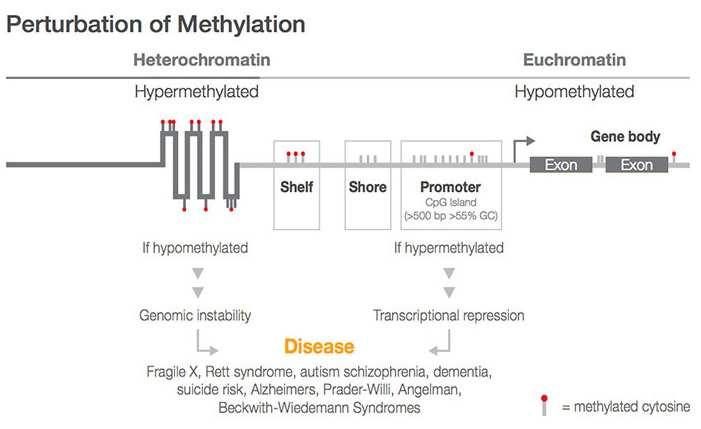
\includegraphics[width=\textwidth]{dna_methylation}
  \caption{
    \url{https://www.illumina.com/techniques/sequencing/methylation-sequencing.html}
    (source)}
\end{figure}

\note{
\begin{itemize}
  \itemsep10pt
  \item ...
\end{itemize}
}

\end{frame}

%%%%%%%%%%%%%%%%%%%%%%%%%%%%%%%%%%%%%%%%%%%%%%%%%%%%%%%%%%%%%%%%%%%%%%%%%%%%%%%%

\begin{frame}[c]{Data analysis? Not yet. Normalization!}

\begin{center}
\begin{itemize}
  \itemsep10pt
  \item Need to normalize the data
  \item Blah blah blah
  \item Images from Rachael
\end{itemize}
\end{center}

\note{
\begin{itemize}
  \itemsep10pt
  \item ...
\end{itemize}
}

\end{frame}

%%%%%%%%%%%%%%%%%%%%%%%%%%%%%%%%%%%%%%%%%%%%%%%%%%%%%%%%%%%%%%%%%%%%%%%%%%%%%%%%

\begin{frame}[c]{Data analysis? Linear Models!}
\begin{center}
\begin{itemize}
  \itemsep10pt
  \item Standard opearting procedure: For each CpG site ($g = 1, \dots, G$), fit
    a linear model:
    \[
      \mathbb{E}[y_g] = X \beta_g
    \]
  \item Test the coefficent of interest using a standard t-test:
    \[
      t_{g} = \frac{\hat{\beta}_{g} - \beta_{g, H_0}}{s_g}
    \]
  \item Such models are a matter of convenience: does $\hat{\beta}_{g}$ really
    answer our questions? Perhaps not.
  \item Is consideration being given to whether the data could have been
    generated by a linear model? Perhaps not.
\end{itemize}
\end{center}

\note{
\begin{itemize}
  \itemsep10pt
  \item CpG sites are thought to function in networks. Treating them as acting
    independently is \textit{not} faithful to the underlying biology.
\end{itemize}
}
\end{frame}

%%%%%%%%%%%%%%%%%%%%%%%%%%%%%%%%%%%%%%%%%%%%%%%%%%%%%%%%%%%%%%%%%%%%%%%%%%%%%%%%%%%%

\begin{frame}[c]{Data analysis? A Data-Adaptive Approach}

\begin{center}
\begin{enumerate}
  \itemsep10pt
  \item Isolate a subset of CpG sites for which there is cursory evidence of
    differential methylation.
  \item Assign CpG sites into neighborhoods --- many ways: genomic distance,
    probe lasso, annotations, etc.
  \item Estimate variable importance measure (VIM) at each screened CpG site,
    using exposure/disease as the intervention ($A$) and with neighboring CpG
    sites in the set of covariates to be controlled for ($W$).
  \item If there are too many neighbors, apply \textit{partitioning around
    medoids} (PAM) to select a subset.
  \item Apply a variant of the Benjamini \& Hochberg FDR procedure, accounting
    for initial screening.
\end{enumerate}
\end{center}

\note{
\begin{itemize}
  \itemsep10pt
  \item Pre-screening is a critical step since we cannot perform computationally
    intensive estimation on...
  \item ...
\end{itemize}
}

\end{frame}

%%%%%%%%%%%%%%%%%%%%%%%%%%%%%%%%%%%%%%%%%%%%%%%%%%%%%%%%%%%%%%%%%%%%%%%%%%%%%%%%

\begin{frame}[c]{Pre-Screening --- Pick Your Favorite Method}

\begin{center}
\begin{itemize}
  \itemsep10pt
  \item The estimation procedure is computationally intensive --- apply it only
    to sites that appear promising.
  \item Consider estimating univariate (linear) regressions of intervention on
    CpG methylation status. Fast, easy.
  \item Select CpG sites with a marginal p-value below, say, $0.01$. Apply
    data-adaptive procedure to this subset.
  \item The modeling assumptions do not matter since the we won't be pursuing
    inference under such a model.
  \item Software implementation is extensible. Users are encouraged to add their
    own. (It's easy!)
\end{itemize}
\end{center}

\note{
\begin{itemize}
  \itemsep10pt
  \item ...
  \item ...
  \item We'll be adding to the available routines for pre-screening too! For
    now, we have \textsc{limma}, and more are on the way.
\end{itemize}
}

\end{frame}

%%%%%%%%%%%%%%%%%%%%%%%%%%%%%%%%%%%%%%%%%%%%%%%%%%%%%%%%%%%%%%%%%%%%%%%%%%%%%%%%

\begin{frame}[c]{Too Many Neighbors? Clustering}

\begin{center}
\begin{itemize}
  \itemsep10pt
  \item There are many options: $k$-means, $k$-medoids, etc., as well as many
    algorithmic solutions.
  \item With limited sample sizes, the number of neighboring sites that may be
    controlled for is limited.
  \item To faithfully answer the question of interest, choose the neighboring
    sites that are the most representative.
  \item This is an \textit{optional} step --- it need only be invoked when there
    are a larger number of CpG sites in the neighborhood.
\end{itemize}
\end{center}

\note{
\begin{itemize}
  \itemsep10pt
  \item ...
  \item ...
  \item ...
\end{itemize}
}

\end{frame}

%%%%%%%%%%%%%%%%%%%%%%%%%%%%%%%%%%%%%%%%%%%%%%%%%%%%%%%%%%%%%%%%%%%%%%%%%%%%%%%%

\begin{frame}[c]{Nonparametric Variable Importance}

\begin{center}
\begin{itemize}
  \itemsep10pt
  \item ...
  \item ...
\end{itemize}
\end{center}

\note{
By allowing scientific questions to inform the parameters that we choose
to estimate, we can do a better job of actually answering the questions of
interest to our collaborators. Further, we abandon the need to specify the
functional relationship between our outcome and covariates; moreover, we
can now make use of advances in machine learning.
}

\end{frame}

%%%%%%%%%%%%%%%%%%%%%%%%%%%%%%%%%%%%%%%%%%%%%%%%%%%%%%%%%%%%%%%%%%%%%%%%%%%%

\begin{frame}[c]{Target Parameters for Complex Questions}

\begin{center}
\begin{itemize}
  \itemsep10pt
  \item Let's consider a simple target parameter: the average treatment effect
    (ATE):
    \[
      \Psi_b(P_0) = \mathbb{E}_{W,0}[\mathbb{E}_0[Y_g \mid A = 1, W_{-g}] -
      \mathbb{E}_0[Y_g \mid A = 0, W_{-g}]]
    \]
  \item No need to specify a functional form or assume that we know the true
    data-generating distribution $P_0$.
  \item Parameters like this can be estimated using \textit{targeted minimum
    loss-based estimation} (TMLE).
  \item \textbf{Asymptotic linearity:}
    \[
      \Psi_b(P_n^*) - \Psi_b(P_0) = \frac{1}{n} \sum_{i = 1}^{n} IC(O_i) +
      o_P\left(\frac{1}{\sqrt{n}}\right)
    \]
\end{itemize}
\end{center}

\note{
Under the additional condition that the remainder term $R(\hat{P}^*, P_0)$
decays as $o_P \left( \frac{1}{\sqrt{n}} \right),$ we have that
$\psi_n - \psi_0 = (P_n - P_0) \cdot D(P_0) + o_P
\left( \frac{1}{\sqrt{n}} \right),$ which, by a central limit theorem,
establishes a Gaussian limiting distribution for the estimator:

$$\sqrt{n}(\psi_n - \psi) \to N(0, V(D(P_0))),$$

where $V(D(P_0))$ is the variance of the efficient influence curve (canonical
gradient) when $\psi$ admits an asymptotically linear representation.

The above implies that $\psi_n$ is a $\sqrt{n}$-consistent estimator of $\psi$,
that it is asymptotically normal (as given above), and that it is locally
efficient. This allows us to build Wald-type confidence intervals in a
straightforward manner:

$$\psi_n \pm z_{\alpha} \cdot \frac{\sigma_n}{\sqrt{n}},$$

where $\sigma_n^2$ is an estimator of $V(D(P_0))$. The estimator $\sigma_n^2$
may be obtained using the bootstrap or computed directly via the following

$$ \sigma_n^2 = \frac{1}{n} \sum_{i = 1}^{n} D^2(\bar{Q}_n^*, g_n)(O_i)$$
}

\end{frame}

%%%%%%%%%%%%%%%%%%%%%%%%%%%%%%%%%%%%%%%%%%%%%%%%%%%%%%%%%%%%%%%%%%%%%%%%%%%%%%%%

\begin{frame}[c]{Corrections for Multiple Testing}

\begin{center}
\begin{itemize}
  \itemsep10pt
  \item ...
  \item ...
\end{itemize}
\end{center}

\note{
\begin{itemize}
  \itemsep10pt
  \item ...
  \item ...
  \item ...
\end{itemize}
}

\end{frame}

%%%%%%%%%%%%%%%%%%%%%%%%%%%%%%%%%%%%%%%%%%%%%%%%%%%%%%%%%%%%%%%%%%%%%%%%%%%%%%%%

\begin{frame}[c]{Software package: R/``methyvim''}

\begin{center}
\begin{itemize}
  \itemsep10pt
  \item ...
  \item ...
\end{itemize}
\end{center}

\note{
\begin{itemize}
  \itemsep10pt
  \item ...
  \item ...
  \item ...
\end{itemize}
}

\end{frame}

%%%%%%%%%%%%%%%%%%%%%%%%%%%%%%%%%%%%%%%%%%%%%%%%%%%%%%%%%%%%%%%%%%%%%%%%%%%%%%%%

\begin{frame}[c]{Data analysis the ``methyvim'' way}

\begin{center}
\begin{itemize}
  \itemsep10pt
  \item ...
  \item ...
\end{itemize}
\end{center}

\note{
\begin{itemize}
  \itemsep10pt
  \item ...
  \item ...
  \item ...
\end{itemize}
}

\end{frame}

%%%%%%%%%%%%%%%%%%%%%%%%%%%%%%%%%%%%%%%%%%%%%%%%%%%%%%%%%%%%%%%%%%%%%%%%%%%%%%%%

\begin{frame}[c]{Review: Summary}

\begin{center}
\begin{itemize}
  \itemsep10pt
  \item Look, we proved this above.
  \item More stuff we proved.
  \item Yet another point here.
  \item Final point goes here.
\end{itemize}
\end{center}

\note{It's always good to include a summary.}

\end{frame}

%%%%%%%%%%%%%%%%%%%%%%%%%%%%%%%%%%%%%%%%%%%%%%%%%%%%%%%%%%%%%%%%%%%%%%%%%%%%%%%%

% don't want dimming with references
\setbeamercovered{}
\beamerdefaultoverlayspecification{}

\begin{frame}[c,allowframebreaks]{References}

\bibliographystyle{apalike}
\nocite{*}
\bibliography{references}

%\note{Here's some work we've talked about. Go check these out if interested.}

\end{frame}

%%%%%%%%%%%%%%%%%%%%%%%%%%%%%%%%%%%%%%%%%%%%%%%%%%%%%%%%%%%%%%%%%%%%%%%%%%%%%%%%

\begin{frame}{Acknowledgments}

\vspace{18pt}

\begin{tabular}{@{}l@{\hspace{1.5cm}}l@{}}
  Mark van der Laan & \footnotesize \lolit University of California, Berkeley \\
  Alan Hubbard \\
  Martyn Smith \\

\\[2ex]

Collaborator, the first & \footnotesize \lolit University or Institution 2 \\
Collaborator, the second \\
\end{tabular}

\vspace{10mm}

Funding source?

\note{
}

\end{frame}

%%%%%%%%%%%%%%%%%%%%%%%%%%%%%%%%%%%%%%%%%%%%%%%%%%%%%%%%%%%%%%%%%%%%%%%%%%%%%%%%

\begin{frame}[c]{Thank you.}

\Large
Slides: \href{https://goo.gl/JDhSEg}{goo.gl/JDhSEg} \quad

\includegraphics[height=5mm]{Figs/cc-zero.png}

\vspace{3mm}
Notes: \href{https://goo.gl/xabp3Q}{goo.gl/xabp3Q}

\vspace{3mm}
Source (repo): \href{https://goo.gl/m5As73}{goo.gl/m5As73}

\vspace{3mm}
\href{https://www.stat.berkeley.edu/~nhejazi}{\tt
  stat.berkeley.edu/\textasciitilde{}nhejazi}

\vspace{3mm}
\href{http://nimahejazi.org}{\tt nimahejazi.org}

\vspace{3mm}
\href{https://twitter.com/nshejazi}{\tt twitter/@nshejazi}

\vspace{3mm}
\href{https://github.com/nhejazi}{\tt github/nhejazi}

\note{Here's where you can find me, as well as the slides for this talk.}

\end{frame}

%%%%%%%%%%%%%%%%%%%%%%%%%%%%%%%%%%%%%%%%%%%%%%%%%%%%%%%%%%%%%%%%%%%%%%%%%%%%%%%%

\end{document}

